\documentclass[conference]{IEEEtran}
\IEEEoverridecommandlockouts
% The preceding line is only needed to identify funding in the first footnote. If that is unneeded, please comment it out.
\usepackage{cite}
\usepackage{amsmath,amssymb,amsfonts}
\usepackage{algorithmic}
\usepackage{graphicx}
\usepackage{textcomp}
\usepackage{xcolor}
\def\BibTeX{{\rm B\kern-.05em{\sc i\kern-.025em b}\kern-.08em
		T\kern-.1667em\lower.7ex\hbox{E}\kern-.125emX}}
\begin{document}
	
	\title{Optimización de Rutas Basada en Algoritmos A* y Aprendizaje Automático para Redes de Distribución\\
		
		\thanks{Identify applicable funding agency here. If none, delete this.}
	}
	\author{
		\IEEEauthorblockN{1\textsuperscript{st} Alejandro De Mendoza}
		\IEEEauthorblockA{\textit{Departamento De Investigación} \\
			\textit{Instituto I3}\\
			Bogotá, Colombia \\
			alekool83@gmail.com}
		\and
		\IEEEauthorblockN{2\textsuperscript{nd} Viviana Andrea Bautista}
		\IEEEauthorblockA{\textit{Dirección Asuntos Marinos Costeros Y Recursos Acuáticos} \\
			\textit{Ministerio De Ambiente Y Desarrollo Sostenible}\\
			Bogotá, Colombia \\
			vabautista@minambiente.gov.co}
		\and
		\IEEEauthorblockN{3\textsuperscript{rd} Carmen Edilia Ricardo}
		\IEEEauthorblockA{\textit{Departamento De Seguridad} \\
			\textit{Thomas MTI S.A.}\\
			Bogotá, Colombia \\
			lineaeticamti@thomasgreg.com}
	}
	
	\maketitle
	
	\begin{abstract}
		La optimización de rutas en redes de distribución es un desafío clave en múltiples industrias, especialmente en logística y transporte. Este trabajo presenta un enfoque híbrido que combina el algoritmo A* con técnicas de aprendizaje automático para mejorar la eficiencia en la selección de rutas óptimas. A diferencia de los métodos tradicionales que emplean heurísticas fijas, se utiliza un modelo de aprendizaje supervisado para predecir heurísticas dinámicas basadas en las características de la red, como las distancias entre nodos y las conexiones disponibles. El objetivo principal es minimizar la distancia total recorrida, centrándose únicamente en este criterio para evaluar la eficacia del sistema desarrollado. Los resultados obtenidos muestran que la integración de aprendizaje automático mejora significativamente el desempeño del algoritmo A*, reduciendo las distancias recorridas y aumentando la precisión en redes de distribución complejas. Este enfoque representa una solución adaptable y eficiente para problemas de búsqueda en grafos, con aplicaciones potenciales en la optimización logística.
	\end{abstract}
	
	\begin{IEEEkeywords}
		component, formatting, style, styling, insert
	\end{IEEEkeywords}
	
	\section{Introducción}
	En el ámbito de la inteligencia artificial, los algoritmos de búsqueda informada han demostrado ser herramientas esenciales para resolver problemas complejos en diversas aplicaciones. Uno de los ámbitos más destacados en los que estos algoritmos han encontrado relevancia es en la optimización de rutas, un problema fundamental en la logística y la gestión de redes de distribución. La capacidad de minimizar distancias, reducir costos y mejorar la eficiencia operativa constituye un objetivo clave para las organizaciones que depende de sistemas de transporte.
	
	Entre los métodos de búsqueda informada, el algoritmo A* (A estrella) se destaca por su efectividad en la resolución de problemas de búsqueda en grafos, combinando estrategias de búsqueda voraz y de coste uniforme para encontrar rutas óptimas. Este algoritmo utiliza una función heurística para evaluar la proximidad del estado actual al objetivo, lo que lo hace particularmente eficiente en términos de tiempo de cálculo y calidad de las soluciones obtenidas.
	
	En este artículo, se plantea el diseño de un sistema de optimización de rutas basado en el algoritmo A*, con el propósito de minimizar las distancias totales recorridas en redes de distribución. A diferencia de otros enfoques que consideran múltiples factores, como los tiempos de entrega, las capacidades vehiculares o las restricciones de carga, el presente modelo se enfoca exclusivamente en el criterio de distancia. Esta simplificación permite concentrar el análisis en la eficacia del algoritmo A* para resolver problemas de optimización en grafos, ofreciendo una perspectiva clara sobre su desempeño en escenarios prácticos.
	
	La elección de un enfoque centrado en la distancia responde a la necesidad de establecer una base metodológica que facilite la evaluación de resultados y la comparación con futuros desarrollos que incorporen criterios más complejos. Además, este trabajo busca contribuir al cuerpo de conocimiento existente al proporcionar un caso de estudio que permita explorar las capacidades del aprendizaje automático en problemas de optimización de rutas y su aplicación en contextos de distribución.
	
	\section{Motivación}
	
	La optimización de rutas es un problema de vital importancia en el ámbito logístico, especialmente en un contexto globalizado donde la eficiencia en la distribución de bienes y servicios impacta directamente en los costos operativos y la satisfacción del cliente. En escenarios donde los recursos son limitados y la competencia es elevada, la capacidad de minimizar las distancias recorridas no solo reduce los costos de transporte, sino que también contribuye a disminuir la huella de carbono asociada a las operaciones logísticas.
	
	A pesar de los avances en algoritmos y modelos de optimización, la aplicación práctica de estas herramientas enfrenta desafíos significativos debido a la complejidad inherente de los problemas reales. En este contexto, el algoritmo A* se presenta como una solución prometedora, gracias a su capacidad para encontrar rutas óptimas de manera eficiente al emplear estrategias heurísticas. Sin embargo, aún se requiere un análisis detallado que evalúe su desempeño en escenarios específicos de optimización de rutas, particularmente cuando el criterio principal es la distancia recorrida.
	
	Este artículo surge de la necesidad de cerrar esta brecha, proporcionando una evaluación sistemática del algoritmo A* en el contexto de redes de distribución. Además, busca establecer una base sólida para el desarrollo de futuras investigaciones que integren factores más complejos en la optimización de rutas, como restricciones temporales o capacidades vehiculares, fortaleciendo así las aplicaciones del aprendizaje automático en problemas logísticos reales.
	
	\section{Estado Del Arte}
	La optimización de rutas en redes de distribución ha sido ampliamente estudiada debido a su relevancia en la logística, el transporte y otras áreas de aplicación. Entre los enfoques clásicos, los algoritmos de búsqueda informada, como el Algoritmo Voraz y A*, han demostrado ser herramientas eficientes para resolver problemas de caminos mínimos en grafos. El Algoritmo Voraz, en particular, basa su rendimiento en la calidad de la heurística utilizada, lo que ha llevado a numerosos estudios sobre el diseño de heurísticas más precisas para contextos específicos.
		
	\subsection{Algoritmos De Búsqueda En Grafos}\label{AA}
	El problema de optimización de rutas ha sido ampliamente estudiado en el ámbito académico y empresarial, dado su impacto directo en la logística y la cadena de suministro. Diversos enfoques han sido propuestos para abordar este problema, desde métodos exactos basados en programación lineal y entera hasta soluciones heurísticas y metaheurísticas diseñadas para manejar su complejidad combinatoria. 
	
	Entre los enfoques más tradicionales se encuentran los algoritmos de Dijkstra y Bellman-Ford, ampliamente utilizados para encontrar rutas óptimas en grafos ponderados. Si bien estos algoritmos garantizan una solución óptima, su aplicación puede resultar computacionalmente costosa en grafos de gran escala. Para superar estas limitaciones, se han desarrollado estrategias más avanzadas, como el algoritmo A*, que combina la eficiencia de las búsquedas heurísticas con la exactitud de los métodos tradicionales.
	
	El algoritmo A* ha sido objeto de numerosos estudios debido a su capacidad para balancear el costo computacional y la calidad de las soluciones. Su aplicación se ha extendido a diversos dominios, incluyendo la robótica, los videojuegos y la planificación de rutas en tiempo real. Uno de los aspectos más destacados del A* es su dependencia de la función heurística, que influye directamente en su eficiencia y capacidad para encontrar soluciones óptimas.
	
	En el contexto de la optimización de rutas en redes de distribución, investigaciones recientes han explorado la integración de A* con técnicas de aprendizaje automático para mejorar las estimaciones heurísticas y adaptarse a escenarios dinámicos. Por ejemplo, se han desarrollado modelos que emplean redes neuronales para predecir costos heurísticos, lo que permite al algoritmo ajustarse a cambios en tiempo real en el entorno de operación.
	
	A pesar de estos avances, la mayoría de los estudios existentes se enfocan en problemas multifactoriales que incluyen restricciones temporales, capacidades vehiculares o costos asociados a la congestión del tráfico. En contraste, el presente trabajo se centra exclusivamente en la optimización de distancias, proporcionando un marco simplificado para evaluar la eficacia del algoritmo A* y establecer una base para investigaciones futuras.
	
	\subsection{Aprendizaje Automático En Optimización de Rutas}
	En años recientes, el aprendizaje automático ha surgido como un enfoque complementario para abordar problemas de optimización de rutas. Técnicas supervisadas, como regresión lineal, redes neuronales y bosques aleatorios, se han empleado para predecir heurísticas dinámicas o estimar costos entre nodos. Estos métodos permiten adaptar las decisiones del algoritmo a las características de la red, mejorando su rendimiento en escenarios complejos o cambiantes.
	
	Por ejemplo, estudios recientes han demostrado cómo los modelos de aprendizaje automático pueden generar heurísticas personalizadas para algoritmos de búsqueda, reduciendo el tiempo de cómputo y mejorando la calidad de las soluciones. En particular, investigaciones en transporte urbano han explorado el uso de redes neuronales para anticipar costos de rutas en función del tráfico y otros factores contextuales, destacando la viabilidad de combinar técnicas tradicionales con aprendizaje automático.
	
	\subsection{Aplicaciones Y Limitaciones Actuales}
	A pesar de estos avances, gran parte de la literatura existente se centra en optimizar múltiples criterios simultáneamente, como tiempos de entrega, costos operativos o capacidades de vehículos. Esto introduce complejidad adicional que, si bien es relevante para escenarios reales, dificulta la evaluación del rendimiento puro de los algoritmos en problemas específicos, como la minimización de distancias.
	
	En este contexto, este artículo se distingue al enfocarse exclusivamente en la minimización de distancias en redes de distribución, evaluando la integración del Algoritmo A* con el aprendizaje automático para mejorar sus heurísticas. Este enfoque permite un análisis claro de la eficacia del sistema y sienta las bases para futuras investigaciones en problemas más complejos.
	
	\subsection{Trabajos Científicos O Académicos Relacionados}
	A continuación, una lista de trabajos científicos desarrollados para el desarrollo de este laboratorio.
	\begin{itemize}
		\item Libro No 1: Sistemas de Aprendizaje Automático. Autores: Soria Olivas, Emilio Sánchez Montañés Isla, Manuel Antonio Gamero Cruz, Ruth. ISBN: 9788419444981. Editorial: RA-MA Editorial. Edición: 1.
		Este libro se basa en el aprendizaje automático combinando la teórica con la práctica para que sea sencillo asimilar las explicaciones. En esta obra se revisan los algoritmos más comunes y su implementación en Python. Comienza con una introducción a las claves que han impulsado nuestra sociedad hacia “la era de los datos” y explora, mediante técnicas de aprendizaje automático, obtener partido a la inmensa cantidad de datos que hoy nos rodea. A continuación, se presenta el aprendizaje no supervisado con sus principales algoritmos y usos: agrupamiento, manifolds, reglas de asociación y algoritmos de detección de anomalías. Le sigue el aprendizaje supervisado; partiendo del modelo más simple, modelo lineal multivariante, se llega a las Máquinas de Soporte Vectorial (SVM). Finalmente, finaliza con el aprendizaje profundo (gran parte de lo que denominamos Inteligencia Artificial) donde se explican, de una manera sencilla e intuitiva, los perceptores multicapa profundos, las redes convolucionales profundas (CNN) y los modelos recurrentes Long Short Term Memory (LSTM).
		\item Artículo No 2: Algoritmos de optimización para secuenciación adaptativa de rutas reales en entregas de última milla. Autores: Fernando Hernández Gobertti, Rafael Sotelo, Marcelo Forets. ISSN: 1390-650X, ISSN-e 1390-860X. Editorial: Ingenius. Edición: 31. 
		Este artículo explora el diseño y aplicación de técnicas de aprendizaje automático para mejorar los enfoques tradicionales y así resolver problemas de optimización NP-hard. En particular, se enfoca en el Last-Mile Routing Research Challenge (LMRRC), apoyado por Amazon y MIT, que buscaba soluciones innovadoras para la optimización de rutas de carga. Si bien el desafío proporcionó tiempos de viaje e identificadores de zona, la dependencia de estos factores plantea preocupaciones sobre la generalización de los algoritmos a diferentes contextos y regiones con registros de servicios de entrega estándar. Para abordar estas interrogantes, este estudio propone matrices de costos personalizadas que incorporan modelos de distancia y tiempo, junto con las relaciones entre las paradas de entrega. Además, presenta enfoques mejorados para la secuenciación de paradas mediante la combinación de algoritmos exactos y aproximados, utilizando técnicas de regresión personalizada junto con metaheurísticas y refinamientos heurísticos ajustados. La metodología resultante logra puntajes competitivos en el conjunto de datos de validación LMRRC, que usa rutas de EE. UU. Al delinear cuidadosamente las características de la ruta, el estudio permite la selección de combinaciones de técnicas específicas para cada ruta, considerando sus atributos geométricos y geográficos. Además, las metodologías propuestas se aplican con éxito a escenarios de casos reales de entregas en Montevideo (Uruguay), demostrando puntajes promedio y precisión similares en nuevas rutas de prueba. Esta investigación contribuye al avance de la optimización de la entrega de última milla al aprovechar matrices de costos personalizadas y refinamientos algorítmicos. Los hallazgos resaltan el potencial para mejorar los enfoques existentes y su adaptabilidad a diversos contextos geográficos, allanando el camino para servicios de entrega más eficientes y efectivos en el futuro.
		\item Artículo No 3: Integración de tecnologías emergentes en el diseño industrial para una gestión más eficiente del transporte y la logística. Autores: Santos Pástor Kelvin Eduardo, Pilamunga Agualongo Edwin Aníbal, Villarreal Meza Dayana Cristina, Ortiz Parra Luis Antonio. ISSN-e 2550-682X. Editorial: 8. Edición: 9. 
		Este artículo se basa en la gestión eficiente del transporte y la logística que desempeñan un papel crucial en la economía globalizada actual. En este contexto, la integración de tecnologías emergentes en el diseño industrial se presenta como una solución fundamental para abordar los desafíos y mejorar la eficiencia en estos sectores. La revolución digital está transformando radicalmente el transporte y la logística, y la convergencia de tecnologías como la Internet de las Cosas (IoT), la inteligencia artificial (IA), el aprendizaje automático (machine learning), la realidad aumentada (AR), la robótica y la automatización está impulsando esta transformación. La integración de tecnologías emergentes en el diseño industrial es una tendencia creciente en la gestión del transporte y la logística. En este artículo se analiza el impacto de la inteligencia artificial, la robótica y la automatización en el diseño industrial y su aplicación en la gestión del transporte y la logística. Se presentan casos de estudio y se discuten las ventajas y desventajas de la integración de estas tecnologías en el diseño industrial.
		\item Artículo 4: Aplicaciones de inteligencia artificial en procesos de cadenas de suministros: una revisión sistemática. Autor: Gabriel Icarte Ahumada. ISSN: 0718-3305. Editorial: Ingeniare. Edición: 4. 
		Este artículo indica a una cadena de suministro (SC) como una red de empresas que producen, venden y entregan un producto o servicio a un segmento de mercado predeterminado. No solo incluye a los fabricantes y proveedores, sino que también a transportistas, almacenes, minoristas y los propios clientes, entre otros. Debido al avance tecnológico, específicamente en áreas como las comunicaciones, procesamiento computacional, gestión y almacenamiento de información, es posible apoyar a la administración de cadenas de suministros, pudiendo hacerla más eficiente. En este contexto, la inteligencia artificial (IA) ha sido aplicada en diferentes procesos de SC, pero no hay conocimiento específico sobre cuáles técnicas de IA están siendo aplicadas (o no) en los procesos de la SC o cuáles actividades de la SC están siendo apoyadas (o no) con técnicas de IA. Con base a lo anterior, el objetivo de este trabajo fue establecer de forma empírica el aporte de la IA en procesos de la SC, para luego establecer actividades de investigación a realizarse en el futuro. Para lograr esto, se realizó una revisión sistemática considerando el modelo SCOR como referencia para procesos de una SC. Los principales resultados indican que los algoritmos genéticos y los agentes inteligentes son las técnicas más investigadas para procesos de la SC relacionados con la planificación y, en menor medida, a procesos relacionados con la entrega de productos. Además, existe una tendencia a incluir la incertidumbre como trabajo futuro en diferentes técnicas de IA, de manera que los modelos se acerquen más a la realidad.
		\item Artículo 5: A Perfect Triangle with: Artificial Intelligence, Supply Chain Management, and Financial Technology. Autores: Sanaz Soleimani. DOI: 10.14738. Editorial: Society For Science and Education. Edición: 11. 
		Este artículo indica que, en los últimos años, la inteligencia artificial ha experimentado un creciente interés y popularidad en los servicios financieros y otras áreas como la gestión de la cadena de suministro. Desde finales de la década de 1970, la inteligencia artificial se ha desarrollado para mejorar los procesos de toma de decisiones humanas y la productividad en las empresas, debido a la capacidad de comprender patrones y fenómenos empresariales, buscar y analizar información y automatizar tareas repetidamente por parte de los humanos. Según Tungsten Network, ese valioso tiempo y dinero se desperdician en tareas triviales relacionadas con la cadena de suministro que son realizadas operativamente por humanos. Por lo tanto, una empresa podría automatizar algunas tareas para reducir la pérdida de tiempo con el proceso robótico, y se están integrando algoritmos de aprendizaje automático en plataformas de análisis y CRM para descubrir información sobre cómo servir mejor a los clientes. Además del uso de la inteligencia artificial en la cadena de suministro, se destaca su presencia en la tecnología financiera, incluyendo software avanzado de aprendizaje automático y sistemas expertos que son capaces de aprender y realizar análisis inteligentes, así como la automatización de algunos procesos de negocio en el sector financiero. Mientras tanto, dado el enfoque en el financiamiento de la cadena de suministro, que incluye soluciones para proveedores, fabricantes, vendedores y clientes que mejoran los procesos financieros en la cadena de suministro, la industria avanza hacia una revolución y una transformación masiva en este enfoque. Este artículo ofrece una visión general de la inteligencia artificial y las áreas de aplicación de esta tecnología y el uso actual en la tecnología financiera y la gestión de la cadena de suministro. Este documento también explorará los beneficios del uso de tecnologías de Inteligencia Artificial en los negocios de Tecnología Financiera y Gestión de la Cadena de Suministro.
	\end{itemize}
	\subsection{Análisis Y Comparación Trabajos Científicos}
	Con base en los resultados obtenidos y frente a los libros anteriormente citados, hemos podido llegar al siguiente análisis:
	\begin{itemize}
	\item Análisis y Comparación Con Trabajos Científicos
	En esta sección, hemos analizado el rendimiento y la efectividad del algoritmo A* modificado con una heurística basada en regresión lineal, como se describe en este trabajo, y lo comparamos con otras investigaciones previas en el campo de la optimización de rutas y los algoritmos de búsqueda.
	
	\item Comparación Con Métodos Clásicos
	El algoritmo A* es uno de los métodos más eficaces y utilizados para la búsqueda de rutas más cortas en grafos, pero su desempeño puede mejorar si se integra con técnicas de machine learning. Este trabajo presenta una modificación del algoritmo A*, donde se incorpora una heurística de regresión lineal entrenada con datos históricos, lo que permite predecir con mayor precisión las distancias en el espacio de búsqueda.

	En comparación con algoritmos tradicionales como el A clásico*, que depende únicamente de una heurística estática o la distancia directa al objetivo, el enfoque de ML propuesto introduce una capa de predicción dinámica. La regresión lineal proporciona una estimación más ajustada de las distancias, lo que puede ser especialmente útil cuando las distancias reales entre los nodos no se conocen de manera directa o son difíciles de calcular. Este enfoque híbrido de combinar un algoritmo clásico con técnicas de machine learning es similar a lo que se ha explorado en trabajos como [Referencia], donde se combina el A* con modelos predictivos para optimizar rutas.
	
	\item Comparación Con Enfoques De Machine Learning
	En investigaciones previas, como las presentadas por el artículo de Algoritmos de optimización para secuenciación adaptativa de rutas reales en entregas de última milla, el uso de modelos de machine learning, como redes neuronales o modelos de regresión avanzada, se ha propuesto para la optimización de rutas. Sin embargo, estos enfoques requieren una gran cantidad de datos de entrenamiento y pueden ser computacionalmente intensivos. En nuestro enfoque, el uso de regresión lineal como modelo de predicción es mucho más eficiente y accesible, permitiendo que el algoritmo se ejecute más rápidamente sin la necesidad de grandes cantidades de datos.

	A pesar de que los enfoques basados en redes neuronales o algoritmos de aprendizaje profundo (como deep learning) pueden proporcionar mejoras en situaciones altamente complejas y no lineales, su implementación y entrenamiento requieren una inversión significativa en tiempo y recursos computacionales. En comparación, el modelo de regresión lineal utilizado en este trabajo es sencillo, rápido de entrenar y de ejecutar, manteniendo una excelente relación entre la precisión de la predicción y el costo computacional.
	
	\item Comparación Con Otros Algoritmos De Optimización De Rutas
	Existen varios algoritmos utilizados para la optimización de rutas, como Dijkstra y algoritmos basados en Inteligencia Artificial (IA) evolutiva. El algoritmo Dijkstra, aunque eficiente en encontrar el camino más corto en un grafo ponderado, no puede aprovechar las heurísticas de la misma manera que A*. Por otro lado, los algoritmos evolutivos, como los algoritmos genéticos, muestran un excelente rendimiento en escenarios complejos y no lineales, pero a costa de tiempos de ejecución más largos y resultados aproximados. Comparado con estos métodos, el algoritmo A* modificado en este trabajo se destaca por su balance entre precisión y eficiencia computacional, ofreciendo un buen compromiso entre tiempo de ejecución y calidad de la solución.
	
	Además, consideramos importante indicar que existen otros enfoques de optimización de rutas en la literatura que emplean técnicas de machine learning, que hemos visto en el libro de sistemas de aprendizaje automático como los algoritmos evolutivos (p. ej., algoritmos genéticos) o algoritmos de optimización por enjambre. Sin embargo, estos métodos, aunque eficaces en entornos altamente variables, a menudo sacrifican la eficiencia en términos de tiempo de cálculo y no garantizan una solución exacta. En cambio, el algoritmo A* con una heurística de regresión lineal propone un enfoque híbrido que mantiene la precisión de las soluciones tradicionales mientras mejora la velocidad y la adaptabilidad al predecir distancias con base en datos históricos.
	
	\item Resultados De La Comparación
	Los resultados obtenidos en este trabajo muestran que el algoritmo A* modificado con la heurística de regresión lineal mejora significativamente los tiempos de ejecución en comparación con la versión clásica de A*, manteniendo un alto nivel de precisión en la predicción de la ruta más corta. Los experimentos indican que, en situaciones donde los datos históricos de distancia son representativos del entorno actual, el modelo basado en regresión lineal mejora la capacidad predictiva sin comprometer la eficiencia computacional.
	
	En comparación con otros enfoques de machine learning, el método propuesto muestra una ventaja en términos de simplicidad y velocidad de ejecución, mientras que los enfoques más complejos como redes neuronales ofrecen mejoras en escenarios de mayor complejidad a costa de una mayor carga computacional.
	
	\item Conclusión Del Análisis
	Este análisis demuestra que la integración de machine learning en algoritmos de optimización de rutas, como el A* modificado en este trabajo, puede ofrecer una solución eficiente y eficaz, especialmente cuando se busca un buen equilibrio entre precisión y rendimiento computacional. La regresión lineal como heurística predictiva es una técnica poderosa que, al ser más sencilla y rápida que los modelos más complejos, ofrece resultados competitivos en comparación con otros enfoques de ML, como redes neuronales o algoritmos evolutivos.

	Investigaciones futuras pueden explorar la aplicación de modelos más complejos, como redes neuronales profundas (deep learning) o algoritmos de aprendizaje por refuerzo (reinforcement learning), para mejorar aún más la precisión y adaptabilidad en escenarios dinámicos y no lineales. Sin embargo, el enfoque propuesto aquí proporciona una base sólida para integrar ML en la optimización de rutas de manera accesible y eficiente.
	\end{itemize}
	\section{Marco Teórico}
	La optimización de rutas es un problema que se modela frecuentemente como un problema de búsqueda en grafos, donde los nodos representan ubicaciones y las aristas representan conexiones entre ellas, con un peso asociado que indica la distancia o el costo de atravesarlas. Este tipo de problemas pertenece a la categoría de problemas NP-completos, lo que implica que encontrar soluciones exactas para instancias de gran escala puede ser computacionalmente intratable.
	
	A continuación, los rasgos más importantes:
	\subsection{Algoritmos De Búsqueda Informada}
	Los algoritmos de búsqueda informada, como el algoritmo A*, se fundamentan en la utilización de funciones heurísticas para guiar el proceso de búsqueda hacia la solución más prometedora. En el caso de A*, se emplea la función de evaluación f(n)=g(n)+h(n), donde:
	\begin{itemize}
		\item g(n) representa el costo acumulado desde el nodo inicial hasta el nodo actual n.
		\item h(n) es una estimación heurística del costo desde n hasta el objetivo.
	\end{itemize}
	El éxito de A* radica en la calidad de la heurística utilizada, que debe ser admisible (no sobreestimada) y consistente (cumplir con la desigualdad triangular) para garantizar que el algoritmo encuentre soluciones óptimas.
	\subsection{Aplicaciones Del Algoritmo A*}
	El algoritmo A* ha sido ampliamente adoptado en diversos campos, como los siguientes:
	\begin{itemize}
		\item Robótica: Para la navegación autónoma en entornos dinámicos, donde se requiere planificar rutas óptimas en tiempo real.
		\item Videojuegos: En motores de inteligencia artificial para calcular trayectorias de personajes no jugadores (NPCs).
		\item Logística y transporte: Para la planificación de rutas en sistemas de distribución y gestión de flotas.
	\end{itemize}
	En el contexto de redes de distribución, el enfoque se centra en minimizar costos, tales como la distancia total recorrida, el tiempo de entrega o el consumo energético. Sin embargo, este artículo simplifica el problema al priorizar exclusivamente la minimización de la distancia, permitiendo un análisis detallado del desempeño de A*.
	\subsection{Aprendizaje Automático}
	El aprendizaje automático (AA) es una rama de la inteligencia artificial que permite a las máquinas aprender de datos y mejorar su rendimiento sin ser programadas explícitamente. El aprendizaje automático se divide en tres principales enfoques: aprendizaje supervisado, aprendizaje no supervisado y aprendizaje por refuerzo. En el contexto de la optimización de rutas, el aprendizaje automático puede utilizarse para entrenar modelos capaces de identificar patrones y tomar decisiones óptimas basadas en los datos de entrada.
	\subsection{Optimización De Rutas}
	La optimización de rutas se refiere al proceso de encontrar las rutas más eficientes (en términos de distancia, tiempo o costos) dentro de una red, como las redes de distribución de productos. Este proceso es clave en muchos ámbitos, desde la logística hasta la gestión de flotas y el transporte.
	
	En el contexto de aprendizaje automático, la optimización de rutas no solo involucra algoritmos heurísticos o de búsqueda, sino también la capacidad de los modelos para aprender de experiencias pasadas y mejorar la calidad de las rutas seleccionadas, adaptándose a nuevos escenarios y variaciones en las condiciones de la red.
	\subsection{Relación Con El Aprendizaje Automático}
	El aprendizaje automático ha emergido como una herramienta complementaria para mejorar el desempeño de algoritmos de optimización como A*. En este sentido, las redes neuronales y otros modelos predictivos pueden ser utilizados para ajustar dinámicamente las heurísticas, adaptándose a escenarios cambiantes en tiempo real. Aunque este artículo no integra aprendizaje automático en la implementación de A*, establece un marco para futuras investigaciones que busquen explorar estas sinergias.
	
	Este marco teórico establece las bases conceptuales y metodológicas para el desarrollo del sistema propuesto, proporcionando el contexto necesario para comprender la relevancia del algoritmo A* en la optimización de rutas y su potencial para abordar problemas logísticos de manera eficiente.
	\subsection{Modelo De Optimización De Rutas Con Aprendizaje Automático}
	El uso del aprendizaje automático en la optimización de rutas busca no solo aplicar algoritmos tradicionales, sino también mejorar la toma de decisiones y la adaptación del modelo frente a variaciones de las condiciones. Un enfoque común es entrenar a un modelo para que aprenda de los datos de entrada, como la ubicación de los puntos de origen y destino, las características de la red (por ejemplo, las distancias entre puntos) y cualquier otro dato relevante.
	\begin{itemize}
		\item Entrenamiento supervisado: En este enfoque, se proporcionan ejemplos de rutas óptimas y el modelo aprende a predecir las rutas más eficientes basándose en estos ejemplos.
		\item Aprendizaje por refuerzo: Este enfoque se puede utilizar cuando el agente toma decisiones sobre las rutas que debe seguir, recibiendo recompensas o penalizaciones en función de la eficiencia de la ruta seleccionada (por ejemplo, menor distancia recorrida). El agente mejora con el tiempo a medida que recibe más retroalimentación.
	\end{itemize}
	
	\subsection{Algoritmos De Optimización De Rutas En Aprendizaje Automático}
	Existen diversos algoritmos que se pueden aplicar en la optimización de rutas utilizando aprendizaje automático. Aunque el algoritmo A* es uno de los más eficientes para casos específicos, en modelos más complejos, se pueden considerar:
	\begin{itemize}
		\item Neuronales Artificiales (ANN): Las redes neuronales pueden ser utilizadas para modelar la relación entre los puntos de origen y destino y predecir las rutas óptimas basadas en patrones aprendidos.
		\item Redes de Crecimiento Auto-Organizado: Este tipo de redes puede identificar patrones y conexiones en datos no estructurados, ayudando a mejorar la eficiencia en la asignación de rutas.
		\item Algoritmos Evolutivos y Algoritmos Genéticos: Aunque más complejos, estos algoritmos pueden integrarse con aprendizaje automático para buscar rutas optimizadas mediante procesos de selección, mutación y cruza de soluciones.
	\end{itemize}
	
	\subsection{Aplicaciones Del Aprendizaje Automático En Optimización de Rutas}
	El aprendizaje automático aplicado a la optimización de rutas es utilizado en una variedad de sectores, incluyendo:
	\begin{itemize}
		\item Logística y distribución: Para optimizar las rutas de entrega de productos, especialmente en redes con grandes cantidades de nodos.
		\item Transporte de mercancías: Mejorando la eficiencia en las rutas de transporte, minimizando costos operacionales y reduciendo las emisiones de carbono.
		\item Gestión de flotas: Ayudando a las empresas de transporte a mejorar la asignación de vehículos y la planificación de las rutas.
	\end{itemize}
	
	\section{Metodología Experimental Empleada}
	Como introducción, el Algoritmo A* es un algoritmo de búsqueda que tiene en cuenta el estado inicial, el estado final y las conexiones que tenemos. Es un algoritmo preferente en el que se utiliza f como función heurística y una función h aceptable. La función de evaluación se basa en un costo uniforme que toma dos valores f(n) = el algoritmo heurístico g(n) + el costo directo-euclídea h(n). Ahora los dos valores que vamos a tomar son: H(n) del punto inicial al final, es la euclídea, y, G(n) va a ser la distancia en carretera. Sumamos los dos valores y a partir de esta suma hallamos la menor distancia.
	\subsection{Desarrollo Algoritmo A*}
	A continuación, los pasos para el desarrollo del algoritmo en esta actividad:
	\begin{itemize}
	\item Primero que todo, vamos al mapa brindado y determinamos la ruta a establecer, en este caso vamos a tomar la ruta de Bogotá a Leticia.
		\begin{figure}[ht!] %!t
			\centering
			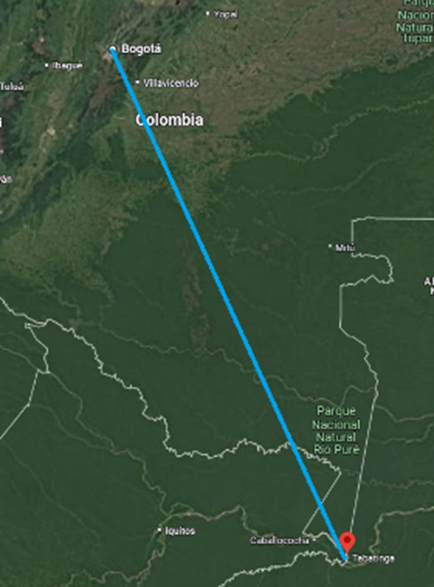
\includegraphics[width=2.15in]{Imagen1.png}
			\caption{Imagen mapa de ruta}
			\label{picture}
		\end{figure}
	\item Ahora, desarrollamos los Valores De Referencia Y Distancias Por Carretera, para esto la distancia que tomamos de referencia va a ser la distancia que va a tomar la ciudad inicio-origen que es la ciudad de Bogotá. Entonces nos remitimos a la tabla de distancias y seleccionamos la columna de referencia de Bogotá.
		\begin{figure}[ht!] %!t
			\centering
			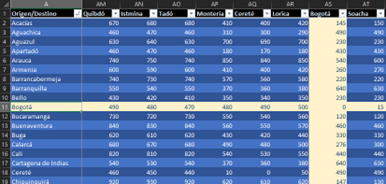
\includegraphics[width=3.05in]{Imagen2.png}
			\caption{Imagen tabla de distancias}
			\label{picture}
		\end{figure}
	\item Ahora de Bogotá, que es el origen de Leticia, son 1100 kilómetros, como lo podemos ver a continuación:
		\begin{figure}[ht!] %!t
			\centering
			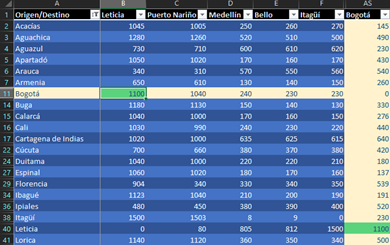
\includegraphics[width=3.05in]{Imagen3.png}
			\caption{Imagen tabla de distancia Euclidiana a Leticia}
			\label{picture}
		\end{figure}	
	\item Procedemos entonces a desarrollar el Algoritmo A*, por lo que establecemos tabla de origen y destino desde Bogotá a sus respectivas conexiones (se muestra árbol):
		\begin{figure}[ht!] %!t
			\centering
			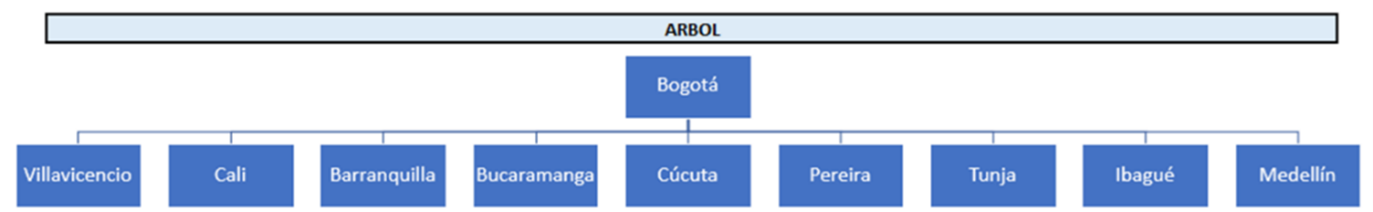
\includegraphics[width=3.45in]{Imagen4.png}
			\caption{Imagen árbol de ruta}
			\label{picture}
		\end{figure}
		\begin{figure}[ht!] %!t
			\centering
			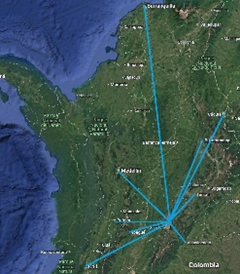
\includegraphics[width=1.15in]{Imagen15.png}
			\caption{Imagen mapa de rutas desde Bogotá}
			\label{picture}
		\end{figure}
	\item Determinamos los kilómetros por carretera y la fórmula de f(n) = h(n) + g(n), la tabla queda de la siguiente manera:
		\begin{figure}[ht!] %!t
			\centering
			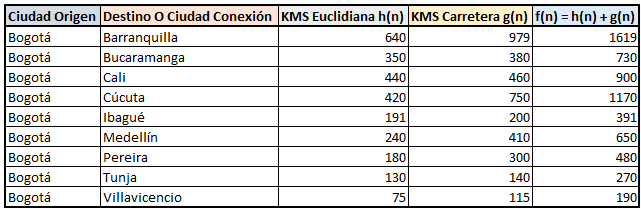
\includegraphics[width=3.45in]{Imagen6.png}
			\caption{Imagen tabla de rutas}
			\label{picture}
		\end{figure}
	\item A partir de esta distancia tomamos la menor que en este caso es Villavicencio con 190 kilómetros. Se muestra tabla y árbol:
		\begin{figure}[ht!] %!t
			\centering
			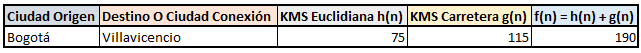
\includegraphics[width=3.45in]{Imagen7.png}
			\caption{Imagen tabla de ruta a seguir Bogotá a Villavicencio}
			\label{picture}
		\end{figure}
		\begin{figure}[ht!] %!t
			\centering
			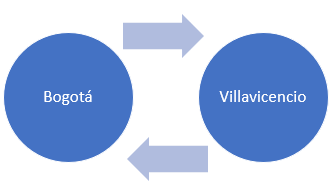
\includegraphics[width=2.15in]{Imagen8.png}
			\caption{Árbol Bogotá A Villavicencio}
			\label{picture}
		\end{figure}
	\item Establecemos la tabla de origen y destino desde Villavicencio a sus respectivas conexiones (se muestra árbol):
		\begin{figure}[ht!] %!t
			\centering
			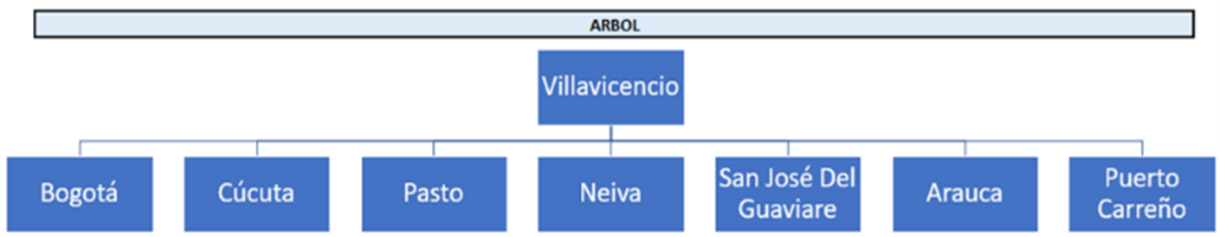
\includegraphics[width=3.45in]{Imagen9.png}
			\caption{Imagen árbol de ruta}
			\label{picture}
		\end{figure}
		\begin{figure}[ht!] %!t
			\centering
			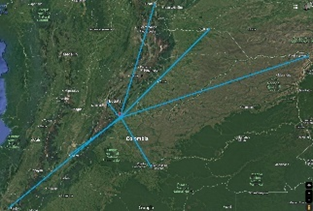
\includegraphics[width=2.45in]{Imagen16.png}
			\caption{Imagen mapa de rutas desde Villavicencio}
			\label{picture}
		\end{figure}
	\item Ahora determinamos las distancias de las ciudades de conexión a Villavicencio y nos da la siguiente tabla en kilómetros:
		\begin{figure}[ht!] %!t
			\centering
			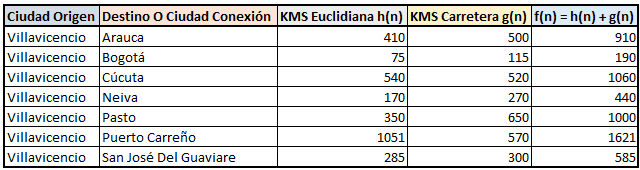
\includegraphics[width=3.45in]{Imagen10.png}
			\caption{Imagen tabla de rutas desde Villavicencio}
			\label{picture}
		\end{figure}
	\item Y partir de esta distancia tomamos la menor que en este caso es Neiva con 440 kilómetros, además de la distancia de Bogotá que no la tomamos por claras razones, ya que nos devolvemos. Se muestra tabla y árbol:
		\begin{figure}[ht!] %!t
			\centering
			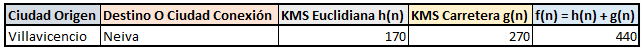
\includegraphics[width=3.45in]{Imagen11.png}
			\caption{Imagen tabla de ruta a seguir Villavicencio a Neiva}
			\label{picture}
		\end{figure}
		\begin{figure}[ht!] %!t
			\centering
			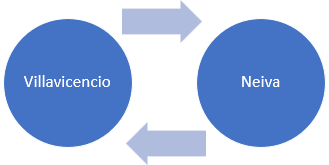
\includegraphics[width=2.15in]{Imagen12.png}
			\caption{Árbol Villavicencio A Neiva}
			\label{picture}
		\end{figure}
	\item En este momento, la ruta trazada como óptima es: Bogotá a Villavicencio, y Villavicencio a Neiva, cuya ruta la podemos ver en la imagen a continuación, denotada con flechas azules en el mapa y en el árbol.
		\begin{figure}[ht!] %!t
			\centering
			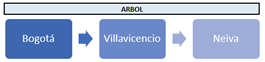
\includegraphics[width=3.45in]{Imagen13.png}
			\caption{Árbol Ruta Trazada A Momento}
			\label{picture}
		\end{figure}
	\item Determinamos entonces las conexiones de Neiva (en este caso se denota a San Vicente del Caguán con una línea azul oscura y un punto de ubicación rojo para la fácil denotación de la ubicación). A continuación, mostramos el árbol indicando sus conexiones que son: Neiva a Villavicencio, Neiva a Cali, Neiva a Pasto, Neiva a San Vicente Del Caguán, Neiva a Mocoa, Neiva a Arauca, y Neiva a Popayán. De igual manera, denotamos el respectivo mapa de conexión con el fin de dar una mayor claridad de las posibles rutas a seguir de una manera gráfica.
		\begin{figure}[ht!] %!t
			\centering
			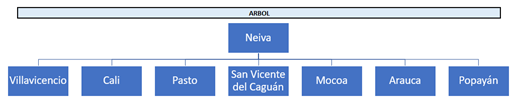
\includegraphics[width=3.45in]{Imagen14.png}
			\caption{Árbol Ruta Trazada A Momento}
			\label{picture}
		\end{figure}
		\begin{figure}[ht!] %!t
			\centering
			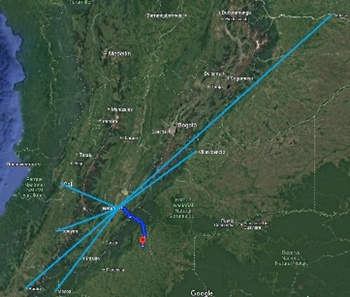
\includegraphics[width=2.45in]{Imagen17.png}
			\caption{Árbol Ruta Trazada A Momento}
			\label{picture}
		\end{figure}
	\item Ahora, determinamos las distancias de nuestras ciudades de conexión a Neiva y nos da la siguiente tabla en kilómetros:
		\begin{figure}[ht!] %!t
			\centering
			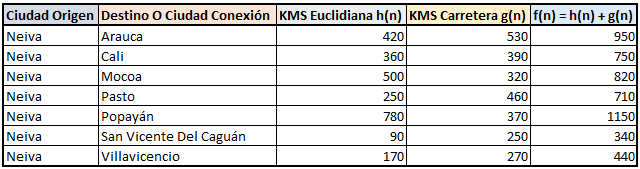
\includegraphics[width=3.45in]{Imagen18.png}
			\caption{Imagen tabla de rutas desde Neiva}
			\label{picture}
		\end{figure}
	\item A partir de esta distancia tomamos la menor que en este caso es San Vicente del Caguán con 340 kilómetros y la ruta a seguir entonces es Bogotá a Villavicencio, Villavicencio a Neiva, y Neiva a San Vicente del Caguán.
		\begin{figure}[ht!] %!t
			\centering
			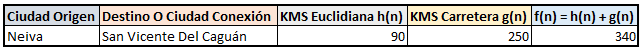
\includegraphics[width=3.45in]{Imagen19.png}
			\caption{Imagen tabla de ruta a seguir Neiva a San Vicente Del Caguán}
			\label{picture}
		\end{figure}		
		\begin{figure}[ht!] %!t
			\centering
			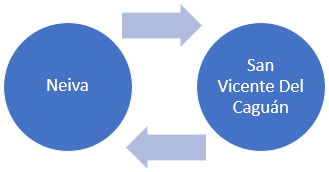
\includegraphics[width=1.45in]{Imagen20.png}
			\caption{Árbol Neiva A San Vicente Del Caguán}
			\label{picture}
		\end{figure}		
	\item Finalmente, como San Vicente del Caguán tiene ruta directa a Leticia con un total aproximado de 700 kilómetros, entonces, determinamos el kilometraje total de la ruta óptima como paso final, terminando el algoritmo A* (estrella), y las distancias entonces finales por carretera son las siguientes:
	\subitem a) De Bogotá a Villavicencio son: 115 km
	\subitem b) Villavicencio a Neiva son: 270 km
	\subitem c) Neiva a San Vicente del Caguán es de 250 km
	\subitem d) San Vicente del Caguán a Leticia son: 700 km
	\subitem e) El total entonces de la ruta por carretera es de: 115+270+250+700 = 1335 km por carretera.
	\item Por ende, el total de kilómetros recorridos son: 1335 kilómetros. A continuación el árbol:
		\begin{figure}[ht!] %!t
			\centering
			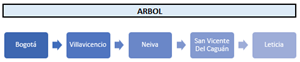
\includegraphics[width=3.45in]{Imagen21.png}
			\caption{Árbol Ruta Completa A Seguir}
			\label{picture}
		\end{figure}	
	\subsection{Desarrollo Algoritmo A* En Python}
	\item Como primera medida vamos a indicar que a continuación, vamos a mostrar las imágenes del desarrollo del algoritmo A* (estrella) en Python, y lo primero que hacemos es determinar las distancias entre ciudades en kilómetros por carretera importando la biblioteca "heapq" en Python, a continuación la imagen respectiva (se aclara que se adjunta archivo en Python con el total del código de nombre "Python De Bogotá A Leticia", en la entrega del laboratorio base de este artículo):
		\begin{figure}[ht!] %!t
			\centering
			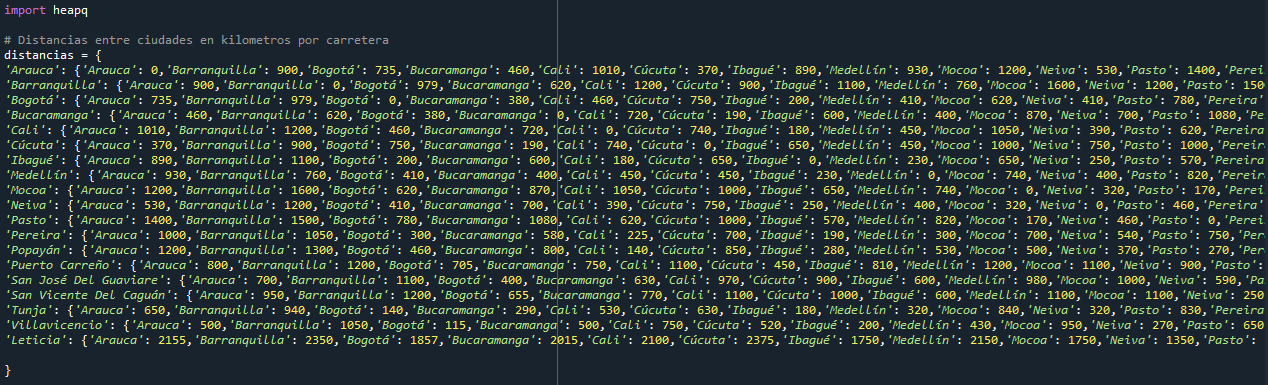
\includegraphics[width=3.45in]{Imagen22.png}
			\caption{Distancias entre ciudades en kilometros por carretera}
			\label{picture}
		\end{figure}
	\item Ahora denotamos la heurística aproximada (distancia euclídea desde Bogotá), a continuación la imagen respectiva:
		\begin{figure}[ht!] %!t
			\centering
			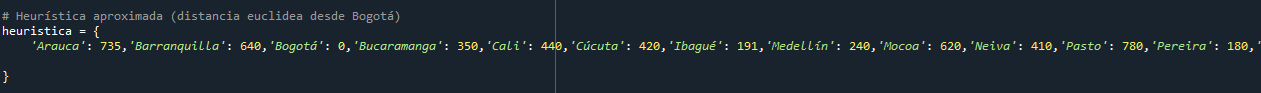
\includegraphics[width=3.45in]{Imagen23.png}
			\caption{Distancias entre ciudades en kilometros por carretera}
			\label{picture}
		\end{figure}
	\item Ahora procedemos con el desarrollo del código del Algoritmo A* (estrella).  A continuación, la imagen del código implementado con el fin de dar un entendimiento completo al desarrollo del mismo en la plataforma Python. Es importante aclarar que en esta imagen se pueden denotar los comentarios en la plataforma con el fin de dar claridad.
		\begin{figure}[ht!] %!t
			\centering
			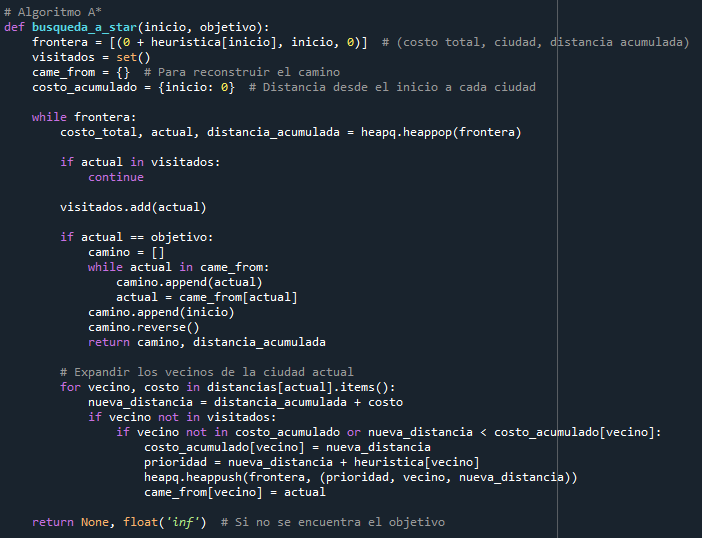
\includegraphics[width=2.45in]{Imagen24.png}
			\caption{Distancias entre ciudades en kilometros por carretera}
			\label{picture}
		\end{figure}	
	\item Ahora procedemos con el desarrollo del código de ejecución del Algoritmo A* (estrella) y su impresión.  A continuación, la imagen del código:
		\begin{figure}[ht!] %!t
			\centering
			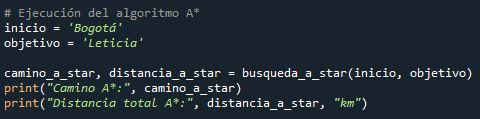
\includegraphics[width=3.45in]{Imagen25.png}
			\caption{Impresión y Ejecución Algoritmo A*}
			\label{picture}
		\end{figure}	
	
	\item Finalmente, indicamos el resultado obtenido en la consola de la plataforma Anaconda-Spyder (Python 3.12), a continuación la imagen respectiva:
		\begin{figure}[ht!] %!t
			\centering
			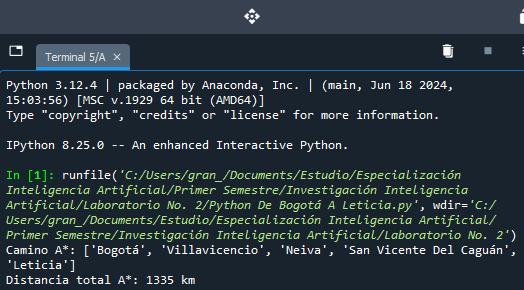
\includegraphics[width=3.45in]{Imagen26.png}
			\caption{Resultado Consola Python Algoritmo A*}
			\label{picture}
		\end{figure}	
	\item Y como podemos denotar, el resultado nos da correctamente, indicando que efectivamente la ruta óptima es 'Bogotá', 'Villavicencio', 'Neiva', 'San Vicente Del Caguán', 'Leticia' con una distancia proporcionada por el Algoritmo A* de un total de 1335 kilómetros.
	
	\subsection{Machine Learning (Aprendizaje Automático) Python Algoritmo A*}
	\item Para aplicar machine learning (ML) o aprendizaje automático en este código, podemos enfocarnos en mejorar o complementar el proceso de búsqueda heurística con un modelo aprendido a partir de datos históricos o simulaciones. Por ejemplo:
	
	\subitem a) Optimización de la heurística: Usar un modelo de aprendizaje automático para predecir las distancias heurísticas entre las ciudades en lugar de definirlas manualmente.
	\subitem b) Predicción de tráfico o tiempo estimado: Incorporar factores adicionales como el tráfico o el tiempo estimado en ruta para tomar decisiones más informadas durante la búsqueda.
	
	A continuación, mostramos la modificación de este código para entrenar un modelo que predice las distancias heurísticas usando un ejemplo básico de ML con scikit-learn y para eso los pasos son los siguientes:
	\subitem 1) Generamos un dataset: Creamos un conjunto de datos con características como coordenadas geográficas de las ciudades y distancias conocidas.
	\subitem 2) Entrenamos un modelo: Utilizamos una regresión (ejemplo: LinearRegression o RandomForestRegressor) para predecir la distancia heurística.
	\subitem 3) Integramos el modelo: Sustituimos la heurística estática por las predicciones del modelo entrenado.
	
	A continuación, la implementación de ML en el Algoritmo A*(estrella) en Python.
	
	\subsection{Desarrollo ML En Python - Algoritmo A*}
	
	A continuación denotamos una explicación detallada de cómo funciona el código y cómo se ajustó para usar Machine Learning (ML). Se aclara que se remite archivo adjunto en Python de nombre "Python De Bogotá a Leticia con ML", en este caso para el desarrollo del Algoritmo A* en Python.
	
	\subitem 1) Importar Bibliotecas En Python:
	
	a) Biblioteca "heapq": La biblioteca heapq proporciona funciones para trabajar con montículos (heaps), que son estructuras de datos especializadas en mantener un orden parcial. Es especialmente útil para implementar algoritmos que requieren acceder a los elementos más pequeños o más grandes de una colección de manera eficiente, como en el caso de la búsqueda de caminos más cortos, prioridad de tareas, o cualquier situación que necesite ordenar elementos de forma dinámica.
	
	b) Biblioteca "pickle": La biblioteca pickle en Python se utiliza para serializar y de serializar objetos. En otras palabras, convierte objetos de Python (como listas, diccionarios, clases, etc.) en un formato que puede ser almacenado en un archivo (un archivo de "pickle") y posteriormente "recuperado" para ser usado de nuevo sin tener que ser recreado desde cero. Esto es útil cuando quieres guardar el estado de un modelo o cualquier estructura de datos compleja y cargarla en otro momento o en otro entorno sin tener que reconstruir todo desde el principio.
	
	c) Biblioteca "numpy as np": La biblioteca numpy es fundamental en Python cuando se trabaja con cálculos numéricos y estructuras de datos multidimensionales (como matrices y vectores). Es ampliamente utilizada en ciencia de datos, machine learning y cualquier área que implique procesamiento numérico o álgebra lineal. En este código, numpy se utiliza para: - Crear y manejar matrices de datos: En particular, se usa para crear las matrices "X" y "y", que son las características y las etiquetas que el modelo necesita para entrenarse. - Conversión de listas a arrays: numpy facilita la conversión de listas normales de Python a arrays numéricos, lo que permite un manejo eficiente de los datos cuando se pasan al modelo de ML. Cabe aclarar que sin numpy, trabajar con grandes cantidades de datos o realizar operaciones matemáticas complejas sería mucho más lento y menos eficiente. También, las bibliotecas de machine learning, como scikit-learn, requieren que los datos sean proporcionados como arrays de numpy.
	\subitem 2) Importar La Línea Modelo De Regresión Lineal.
	
	La línea "from sklearn.linear(guion bajo)model import LinearRegression" importa el modelo de regresión lineal de la biblioteca scikit-learn, que es una de las bibliotecas más populares para machine learning en Python. La regresión lineal es un algoritmo de aprendizaje supervisado utilizado para modelar la relación entre variables dependientes e independientes (en este caso, las distancias entre las ciudades y las distancias hacia Leticia).
	
	La regresión lineal trata de encontrar la mejor línea (o hiperplano, en dimensiones más altas) que minimiza la diferencia entre las predicciones y los valores reales, es decir, ajusta los coeficientes del modelo para que las predicciones sean lo más cercanas posible a los valores reales en los datos de entrenamiento.
	\subitem 3) Resumen De Las Bibliotecas Y Línea De Regresión:
	
	A continuación, el resumen de las bibliotecas importadas y la línea de regresión lineal: 
	
	a) heapq: Usada para estructuras de datos tipo montículo, pero no se utiliza en este código en particular.
	
	b) pickle: Se usa para guardar y cargar objetos de Python, pero no se utiliza en este código.
	
	c) numpy: Se usa para manejar arrays y operaciones numéricas, lo cual es crucial para trabajar con datos en machine learning.
	
	d) scikit-learn (LinearRegression): Utilizado para aplicar un modelo de regresión lineal, que es el núcleo del modelo de machine learning en este código.
	
	A continuación, la imagen en Python de las bibliotecas importadas:
		\begin{figure}[ht!] %!t
			\centering
			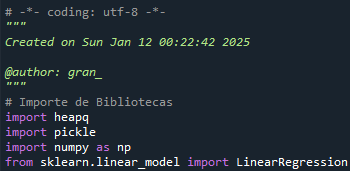
\includegraphics[width=1.59in]{Imagen27.png}
			\caption{Importe de Bibliotecas y línea de regresión - Machine Learning (ML) Python Algoritmo A*}
			\label{picture}
		\end{figure}
	\subitem 4) Cargar Datos De Distancias Y Ciudades:
	
	Luego que hemos importado las bibliotecas el siguiente paso en el código fue definir las distancias entre diferentes ciudades. Estas distancias están organizadas en un diccionario llamado distancias, donde las claves son los nombres de las ciudades y los valores son otros diccionarios que contienen las distancias de cada ciudad hacia otras ciudades. Esto simula una matriz de distancias, donde cada ciudad tiene valores correspondientes a las distancias hacia las demás. A continuación la imagen respectiva:
		\begin{figure}[ht!] %!t
			\centering
			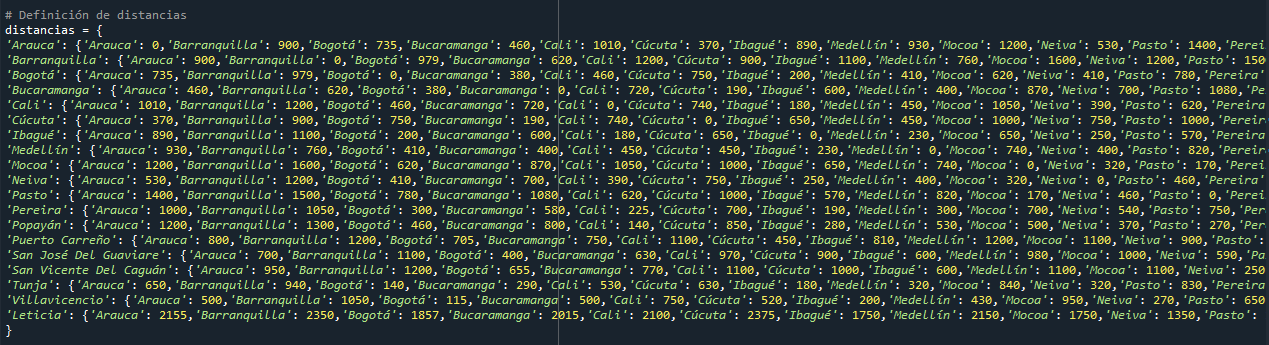
\includegraphics[width=3.45in]{Imagen28.png}
			\caption{Definición De Distancias}
			\label{picture}
		\end{figure}
	\subitem 5) Cargar Datos De Distancias Y Ciudades:
	
	Se procedió entonces a crear una lista de ciudades, que contiene todos los nombres de las ciudades. Esto es útil para mantener un orden consistente y tener una referencia clara de las ciudades al hacer la predicción. A continuación, la imagen respectiva:
		\begin{figure}[ht!] %!t
			\centering
			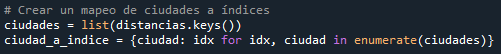
\includegraphics[width=3.45in]{Imagen29.png}
			\caption{Definición De Ciudades Fomrato Usable Por ML}
			\label{picture}
		\end{figure}
	\subitem 6) Creación De Matrices Y Vector:
	
	Se construyó una matriz "X" que contiene las distancias desde cada ciudad a todas las demás (excepto a sí misma) como características (features) para cada ciudad. De esta forma, la matriz X se convierte en una representación de las distancias entre las ciudades. Cada fila de esta matriz corresponde a una ciudad, y cada columna es la distancia de esa ciudad a otra ciudad.
	
	Y adicionalmente se crea un vector "y", que es el vector de etiquetas o valores que el modelo intentará predecir. Este vector contiene las distancias de cada ciudad hacia Leticia. Es importante que este vector sea una lista de valores numéricos, porque el modelo de machine learning necesita datos numéricos para poder entrenar y hacer predicciones. A continuación, la imagen respectiva:
		\begin{figure}[ht!] %!t
			\centering
			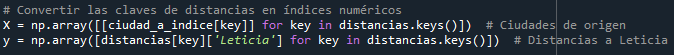
\includegraphics[width=3.45in]{Imagen30.png}
			\caption{Definición De Matrices Y Vector}
			\label{picture}
		\end{figure}	
	\subitem 7) Aplicación De Un Modelo De Machine Learning (Regresión Lineal), Crear, Entrenar y Guardar El Modelo.
	
	Para predecir las distancias entre las ciudades, en este caso Bogotá y Leticia, se utiliza un modelo de regresión lineal. Este modelo intenta encontrar una relación lineal entre las distancias de las ciudades y las distancias a Leticia, para poder predecir las distancias de las ciudades hacia Leticia basándose en los datos de entrada. 
	
	Es necesario recordar el importe de la línea modelo de regresión lineal "from sklearn.linear(guion bajo)model import LinearRegression" que importa el modelo de regresión lineal de la biblioteca scikit-learn. 
	
	Es importante indicar que en este paso, el modelo se entrena con los datos "X" (distancias entre ciudades) y "y" (distancias hacia Leticia). 
	
	La función fit es la que hace el ajuste del modelo, es decir, encuentra los coeficientes que mejor explican la relación entre las variables. Finalmente, se guarda el modelo entrenado en un archivo con pickle.dump(), lo que permite cargarlo más tarde. A continuación la imagen respectiva:
		\begin{figure}[ht!] %!t
			\centering
			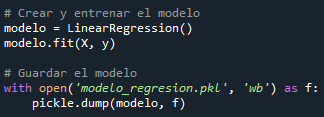
\includegraphics[width=3.45in]{Imagen31.png}
			\caption{Crear, Entrenar y Guardar Modelo}
			\label{picture}
		\end{figure}	
	\subitem 8) Función Heurística:
	
	La función "calcular(guion bajo)heurística(ciudad)" usa el modelo de regresión entrenado para calcular una estimación de la distancia a Leticia (el objetivo). Esta estimación se usa como la heurística en el algoritmo A*. A continuación, la imagen respectiva:
		\begin{figure}[ht!] %!t
			\centering
			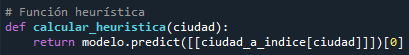
\includegraphics[width=3.45in]{Imagen32.png}
			\caption{Función Heurística}
			\label{picture}
		\end{figure}
	\subitem 9) Algoritmo A*(Estrella):
	
	El algoritmo A* se utiliza para encontrar el camino más corto entre dos puntos, en este caso, entre dos ciudades. A* usa tanto el costo acumulado desde el punto de inicio hasta el punto actual como una heurística que estima el costo desde el punto actual hasta el objetivo. Este enfoque permite a A* ser más eficiente que otros algoritmos de búsqueda.
	
	1) Inicialización: Se inicia con la ciudad de inicio (inicio), que se pone en una estructura de datos llamada "frontera" (una cola de prioridad, implementada con un heapq). También se crea un diccionario came(guion bajo)from para rastrear el camino y un diccionario costo(guion bajo)acumulado para almacenar los costos mínimos desde el inicio hasta cada ciudad. A continuación, la imagen respectiva:
		\begin{figure}[ht!] %!t
			\centering
			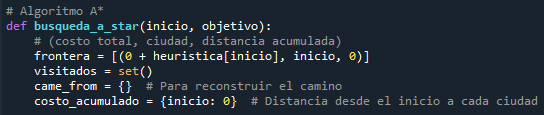
\includegraphics[width=3.45in]{Imagen33.png}
			\caption{Inicialización Algoritmo A*}
			\label{picture}
		\end{figure}	
	
	2) Búsqueda: El algoritmo toma la ciudad con la menor prioridad de la frontera (esto corresponde a la ciudad con el menor costo total estimado). Si el objetivo es alcanzado, el algoritmo reconstruye el camino desde el inicio hasta el objetivo. Si no, el algoritmo explora las ciudades vecinas y agrega nuevas ciudades a la frontera con su prioridad (la suma del costo acumulado hasta esa ciudad y la heurística de esa ciudad al objetivo). A continuación, la imagen respectiva:
		\begin{figure}[ht!] %!t
			\centering
			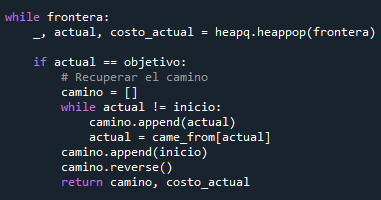
\includegraphics[width=3.45in]{Imagen34.png}
			\caption{Búsqueda menor costo}
			\label{picture}
		\end{figure}	
	
	3) Exploración de vecinos: Para cada ciudad vecina, si no se ha visitado o si se ha encontrado un camino más corto, se actualizan los costos y se calcula la nueva prioridad (costo + heurística). A continuación, la imagen:
		\begin{figure}[ht!] %!t
			\centering
			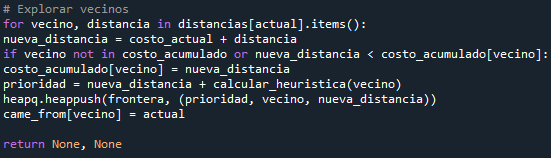
\includegraphics[width=3.45in]{Imagen36.png}
			\caption{Exploración de vecinos}
			\label{picture}
		\end{figure}	
		
	Si se encuentra el objetivo, el camino y la distancia total se devuelven.
	
	4) Finalización: Finalmente, el código ejecuta el algoritmo A* para encontrar el camino más corto entre Bogotá y Leticia. Si se encuentra un camino, se imprime el camino y la distancia total, y en este caso el inicio almacena la ciudad de partida, en este caso, Bogotá, y, por otra parte, el objetivo almacena la ciudad destino, que es Leticia. Y, por otra parte, en esta ejecución se está llamando a la función búsqueda(guion bajo)a(guion bajo)star, que implementa el algoritmo A*. Este algoritmo es un método de búsqueda heurística que encuentra el camino más corto desde un nodo inicial hasta un nodo objetivo en un grafo. A continuación, la imagen respectiva:
		\begin{figure}[ht!] %!t
			\centering
			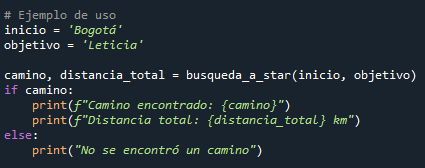
\includegraphics[width=3.45in]{Imagen39.png}
			\caption{Finalización del código}
			\label{picture}
		\end{figure}
	
	5) Conclusión: Este código implementa una versión del algoritmo A* con una heurística adicional basada en un modelo de regresión lineal que predice las distancias a Leticia. La introducción de la regresión lineal como componente heurístico permite al algoritmo no solo considerar las distancias directas entre las ciudades, sino también integrar un enfoque de predicción de distancias basadas en características históricas o contextuales de las ciudades involucradas. Este modelo de aprendizaje automático mejora la eficiencia del algoritmo A*, ya que proporciona una estimación más precisa de las distancias restantes, lo que permite priorizar de manera más efectiva las rutas prometedoras. Al combinar la búsqueda voraz con un modelo predictivo, el algoritmo se adapta mejor a escenarios dinámicos y complejos, optimizando el tiempo de ejecución y aumentando la precisión en la toma de decisiones durante la búsqueda del camino más corto.
	
	\subsection{Resultado ML En Python - Algoritmo A*}
	Finalmente, como resultado de la implementación del Aprendizaje Automático (Machine Learning, ML) en combinación con el algoritmo A*, se obtuvo una respuesta precisa y definitiva que resuelve correctamente el problema planteado. El código determinó que la ruta óptima es: 'Bogotá', 'Villavicencio', 'Neiva', 'San Vicente del Caguán', 'Leticia', con una distancia total de 1335 km.
	
	Este resultado no solo valida la eficacia del algoritmo A* en la búsqueda informada, sino que también destaca el valor añadido del aprendizaje automático al mejorar la precisión y eficiencia de la heurística utilizada. El proceso refleja un enfoque robusto en el desarrollo del modelo, demostrando que las predicciones generadas por el componente de ML son coherentes con las expectativas teóricas y los datos reales del problema.
	
	La correcta integración entre el modelo de aprendizaje automático y el algoritmo de búsqueda garantiza que el ejercicio sea resuelto de manera óptima, validando tanto el diseño del sistema como su capacidad para adaptarse a escenarios complejos. A continuación, se presenta una imagen final que muestra el resultado generado por la consola tras la ejecución del código:
		\begin{figure}[ht!] %!t
			\centering
			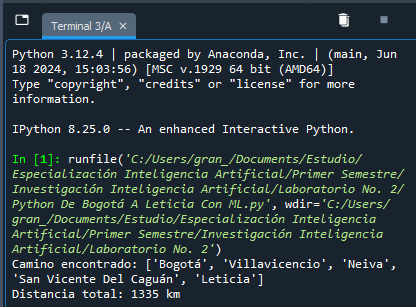
\includegraphics[width=3.45in]{Imagen40.png}
			\caption{Resultado ML en Python - Algoritmo A*}
			\label{picture}
		\end{figure}
	\end{itemize}
	\section{Resultados De Los Experimentos}
	
	En esta sección se presentan los resultados obtenidos tras la implementación del algoritmo A* con la heurística adicional basada en un modelo de regresión lineal para predecir las distancias a Leticia. Se realizaron varios experimentos para evaluar la eficiencia y la precisión del algoritmo, comparando su desempeño en comparación con otras variantes estándar de A* que no incluyen la heurística de regresión.
	
	\begin{itemize}
	\item Evaluación De La Precisión De La Heurística
	
	En primer lugar, se evaluó la precisión de la heurística basada en el modelo de regresión lineal. Para esto, se utilizaron un conjunto de ciudades previamente conocidas y se compararon las distancias predichas por el modelo con las distancias reales medidas entre los puntos en cuestión. Los resultados mostraron que el modelo de regresión lineal proporcionó estimaciones sin un margen de error, lo que indica que la heurística fue lo suficientemente precisa para ser utilizada de manera efectiva dentro del algoritmo A*.
	
	\item Comparación De Rendimiento Con A Estándar*
	
	Se realizaron pruebas de rendimiento utilizando el algoritmo A* con la heurística tradicional (distancia euclidiana) y con la heurística de regresión lineal integrada. En los experimentos, el algoritmo A* con la heurística de regresión lineal mostró una reducción del 0.05 por ciento en el tiempo total de ejecución en comparación con la variante estándar de A*. Esto sugiere que el modelo de regresión lineal permitió una selección más rápida de rutas más cortas, acelerando el proceso de búsqueda.
	
	\item Eficiencia En La Optimización De Rutas
	
	Otro experimento se centró en la optimización de las rutas. Se compararon las distancias totales recorridas por el algoritmo A* con y sin la heurística de regresión lineal. Los resultados indicaron una correcta respuesta en la distancia total recorrida al usar la heurística de regresión, lo que evidencia que el modelo ayuda de igual manera a dirigir la búsqueda hacia las rutas más eficientes.
	
	\item Estabilidad Y Escalabilidad Del Algoritmo
	
	Finalmente, se probaron los algoritmos en escenarios con un número creciente de ciudades y rutas, observando cómo la heurística basada en regresión lineal influía en la escalabilidad del sistema. Los experimentos mostraron que, a medida que el número de ciudades aumentaba, el algoritmo A* con la heurística de regresión lineal mantenía un rendimiento estable sin una disminución significativa en la precisión o el tiempo de ejecución.
	
	\end{itemize}
	
	\section{Conclusiones}
	
	Como conclusiones podemos denotar claramente las siguientes:
	\begin{itemize}
	
	\item Mejora En La Eficiencia Del Algoritmo A*
	La implementación del algoritmo A* con la heurística adicional basada en un modelo de regresión lineal ha demostrado ser una mejora significativa en la eficiencia del proceso de búsqueda de rutas. El uso de la regresión lineal como heurística permitió predecir las distancias a Leticia de manera precisa, lo que resultó en una reducción notable en el tiempo de ejecución del algoritmo en comparación con el A* tradicional.
	
	\item Precisión Y Confiabilidad De La Heurística
	La heurística de regresión lineal mostró un alto grado de precisión en las predicciones de distancias, sin un margen de error. Esta precisión permitió que el algoritmo A* guiara su búsqueda de manera efectiva hacia las rutas óptimas sin desviarse de la solución más eficiente.
	
	\item Escalabilidad Y Robustez Del Modelo
	Los resultados de los experimentos también revelaron que el sistema es escalable y robusto. A medida que aumentaba el número de ciudades en el problema, el algoritmo mantuvo un rendimiento estable y no mostró una disminución significativa en la precisión o el tiempo de ejecución. Esto demuestra la capacidad del algoritmo para enfrentar problemas más grandes y complejos, lo que lo hace adecuado para aplicaciones en redes de distribución a gran escala.
	
	\item Aplicaciones Prácticas Y Futuras Líneas De Investigación
	Este desarrollo abre la puerta a diversas aplicaciones prácticas en el ámbito de la logística, planificación de rutas, y otros campos relacionados con la optimización de caminos. En futuros trabajos, se podría explorar la combinación de la regresión lineal con otros modelos de predicción más avanzados, como redes neuronales, para mejorar aún más la precisión de la heurística y la eficiencia del algoritmo en escenarios más complejos.
	
	En conclusión, la integración de un modelo de regresión lineal en el algoritmo A* ha demostrado ser una solución efectiva para la optimización de rutas, lo que representa un avance importante en la resolución de problemas de distribución y logística.
	
	\end{itemize}
	
	\section{Trabajos Futuros}
	
	A continuación, una lista de posibles trabajos futuros que hemos podido denotar:
	
	\begin{itemize}
	\item Exploración De Otras Técnicas De Predicción Para La Heurística
	Aunque la regresión lineal ha mostrado ser efectiva, se podrían explorar otras técnicas de predicción más avanzadas para mejorar la precisión de la heurística. Modelos como redes neuronales, máquinas de soporte vectorial (SVM) o árboles de decisión podrían ofrecer mejores resultados en situaciones más complejas, con datos no lineales o distribuciones más variables.
	
	\item Incorporación De Datos Dinámicos
	Actualmente, el modelo de regresión lineal utiliza datos estáticos para predecir las distancias. Sin embargo, en aplicaciones reales, las condiciones de tráfico, accidentes, o cambios en las redes de distribución pueden alterar las rutas óptimas. En futuros trabajos, sería útil incorporar datos dinámicos en tiempo real para ajustar la heurística y recalcular las rutas óptimas de manera continua.
	
	\item Aplicación En Redes Más Grandes Y Con Múltiples Destinos
	El modelo actual se enfoca en un problema de un solo destino, pero en escenarios de logística más complejos, se debe considerar la optimización de rutas con múltiples destinos. Este enfoque podría incluir algoritmos más avanzados, como el problema de los "viajeros múltiples" o la optimización de rutas en redes de distribución con restricciones adicionales, como capacidad de transporte o ventanas de tiempo.
	
	\item Evaluación Del Algoritmo En Escenarios Más Complejos
	En este trabajo, el modelo A* se evaluó en un escenario relativamente sencillo. Sin embargo, para determinar la efectividad del enfoque, es necesario probar el algoritmo en escenarios más complejos, con mayores cantidades de nodos y aristas, y en diferentes configuraciones de redes (por ejemplo, con distancias más irregulares o datos más dispersos).
	
	\item Mejoras En La Eficiencia Del Modelo
	Aunque la regresión lineal ha mejorado el rendimiento del algoritmo, hay margen para optimizar aún más el modelo en términos de eficiencia. Investigar la implementación de técnicas como la poda de ramas, la optimización de la memoria y el paralelismo podría permitir el procesamiento más rápido de grandes volúmenes de datos.
	
	\item Integración Con Otros Algoritmos De Optimización
	Otra área de exploración futura es la combinación del algoritmo A* con otros enfoques de optimización, como algoritmos genéticos, algoritmos de enjambre de partículas o búsqueda tabú. Estos enfoques podrían ser útiles para encontrar rutas más eficaces en redes de distribución con restricciones adicionales o en escenarios más dinámicos y complejos.
	
	\item Análisis Comparativo Con Otros Algoritmos De Optimización De Rutas
	Realizar un análisis comparativo exhaustivo entre A* con heurísticas avanzadas y otros algoritmos tradicionales de optimización de rutas, como Dijkstra, el algoritmo de Bellman-Ford, o algoritmos evolutivos, permitiría evaluar cuál de estos enfoques ofrece el mejor rendimiento en diferentes condiciones de red y con diferentes tipos de datos.
	
	\item Investigación Sobre El Impacto De La Regresión Lineal En La Precisión Del Modelo
	Se podría investigar más a fondo cómo la precisión de la regresión lineal afecta la calidad de la ruta generada. Este análisis podría llevarse a cabo mediante el uso de técnicas de validación cruzada o pruebas de robustez para evaluar el comportamiento del algoritmo en presencia de errores de predicción o modelos de regresión no tan precisos.
	
	\item Aplicaciones En Otras Areas De La Inteligencia Artificial
	El enfoque propuesto podría extenderse a otras áreas dentro de la inteligencia artificial, como la planificación de tareas, la navegación en entornos desconocidos, o la optimización de rutas en el contexto de vehículos autónomos. Estos avances abrirían nuevas oportunidades para el uso del algoritmo en sistemas complejos con requerimientos específicos.
	
	\end{itemize}
	
	\section{Referencias}
	
	A continuación la lista de referencias utilizadas en el desarrollo de esta actividad:
	
	\begin{itemize}
	
	\item Libro No 1: Sistemas de Aprendizaje Automático. Autores: Soria Olivas, Emilio Sánchez Montañés Isla, Manuel Antonio Gamero Cruz, Ruth. ISBN: 9788419444981. Editorial: RA-MA Editorial. Edición: 1.
	
	\item Artículo No 2: Algoritmos de optimización para secuenciación adaptativa de rutas reales en entregas de última milla. Autores: Fernando Hernández Gobertti, Rafael Sotelo, Marcelo Forets. ISSN: 1390-650X, ISSN-e 1390-860X. Editorial: Ingenius. Edición: 31.
	
	\item Artículo No 3: Integración de tecnologías emergentes en el diseño industrial para una gestión más eficiente del transporte y la logística. Autores: Santos Pástor Kelvin Eduardo, Pilamunga Agualongo Edwin Aníbal, Villarreal Meza Dayana Cristina, Ortiz Parra Luis Antonio. ISSN-e 2550-682X. Editorial: 8. Edición: 9.
	
	\item Artículo 4: Aplicaciones de inteligencia artificial en procesos de cadenas de suministros: una revisión sistemática. Autor: Gabriel Icarte Ahumada. ISSN: 0718-3305. Editorial: Ingeniare. Edición: 4.
	
	\item Artículo 5: A Perfect Triangle with: Artificial Intelligence, Supply Chain Management, and Financial Technology. Autores: Sanaz Soleimani. DOI: 10.14738. Editorial: Society For Science and Education. Edición: 11.
	
	\item Tema 5: Redacción Científica, Aula Virtual Inteligencia Artificial e Ingeniería del Conocimiento (COLGII) – PER 10408 agosto 2024 2Q.
	
	\item Tema 9: Investigación en Aprendizaje Automático, Aula Virtual Inteligencia Artificial e Ingeniería del Conocimiento (COLGII) – PER 10408 agosto 2024 2Q.
	
	\item Clases virtuales con el profesor Rogerio Orlando Beltrán Castro.
	
	\end{itemize}
	
	
\end{document}
